\chapter{Geladenes Teilchen im elektrischen Feld\label{chapter:efeld}}
\lhead{Teilchen im elektrischen Feld}
\begin{refsection}
\chapterauthor{Michael Cerny und Stefan Schindler}


In diesem Kapitel erweitern wir das Beispiel des Potentialkastens 
(Kapitel \ref{subsection:potentialkasten}, Seite \pageref{subsection:potentialkasten})
um eine St\"orung.

\section{St"orungstheorie}
Grunds"atzlich k"onnen wir mit der St\"orungstheorie ein einfaches Modell 
(Abb \ref{abb:efeld_psi_ungestoert} der ersten 5 Energieniveaus) 
mit einer St\"orung erg"anzen, statt von Anfang an mit einem komplexen Modell zu rechnen.

Allgemein gilt:
\[
  f(x, \varepsilon) = f_0(x) + \varepsilon*f_1(x) + \varepsilon^2*f_2(x) + \ldots + \varepsilon^\infty*f_\infty(x)
\]
Dabei ist $f_0(x)$ die urspr\"ungliche Funktion und $f_n(x)$ die $n$-te  N"aherung der St"orung.
Mit $\varepsilon$ wird die St"orung gesteuert. Dabei sollte $\varepsilon$ nicht zu gross gew"ahlt werden, 
da die N"aherung sonst ungenau wird. 

Setzen wir $\varepsilon = 0$, k\"onnen wir die St"orung dynamisch abschalten.

In der Quantenmechanik k"onnen wir die St"orungstheorie anwenden indem wir den Hamilton-Operator der 
urspr"unglichen Funktion $H_0$ um zus"atzliche $\varepsilon^n*H_n$ erg"anzen:
\[
  H = \varepsilon^0*H_0 + \varepsilon^1*H_1 + \varepsilon^2*H_2 + \ldots + \varepsilon^\infty \hat H_\infty
\]












\section{Anwendungen}

\subsection{Potentialkasten mit eFeld}


\subsubsection{Modell der St\"orung elektrisches Feld}

In diesem Modell wollen wir den Grundzustand mit einem elektrischen Feld st\"oren.

Diese St\"orung heisst in der 1. N\"aherung $\hat H_1$ \& wird wie die gesamte St"orung \"uber den 
Parameter $\varepsilon$ gesteuert.

$V_1$ wird als lineares Feld definiert:
\begin{equation}
  V_1(x) = a*x + b
\end{equation}

Der Parameter $a$ steht f\"ur die Feldst\"arke, der Parameter $b$ f\"ur die Grundspannung.

Da wir $a$ jedoch bereits durch $\varepsilon$ beschreiben, k\"onnen wir mit $a = 1$ vereinfachen.

F\"ur die Berechnung ist es einfacher das Feld symetrisch anzulegen. Darum setzen wir $b = 0$ \& reduzieren:
\[
  V_1(x) = x
\]

Eingesetzt wird daraus:

\[
  \hat{H} = \varepsilon^0 ( \frac{\hbar^2}{2m} \frac{\partial^2}{\partial x^2} + V_0(x) )
            + \varepsilon^1 ( \frac{\hbar^2}{2m} \frac{\partial^2}{\partial x^2} + x )
\]


\begin{figure}
 \centering
 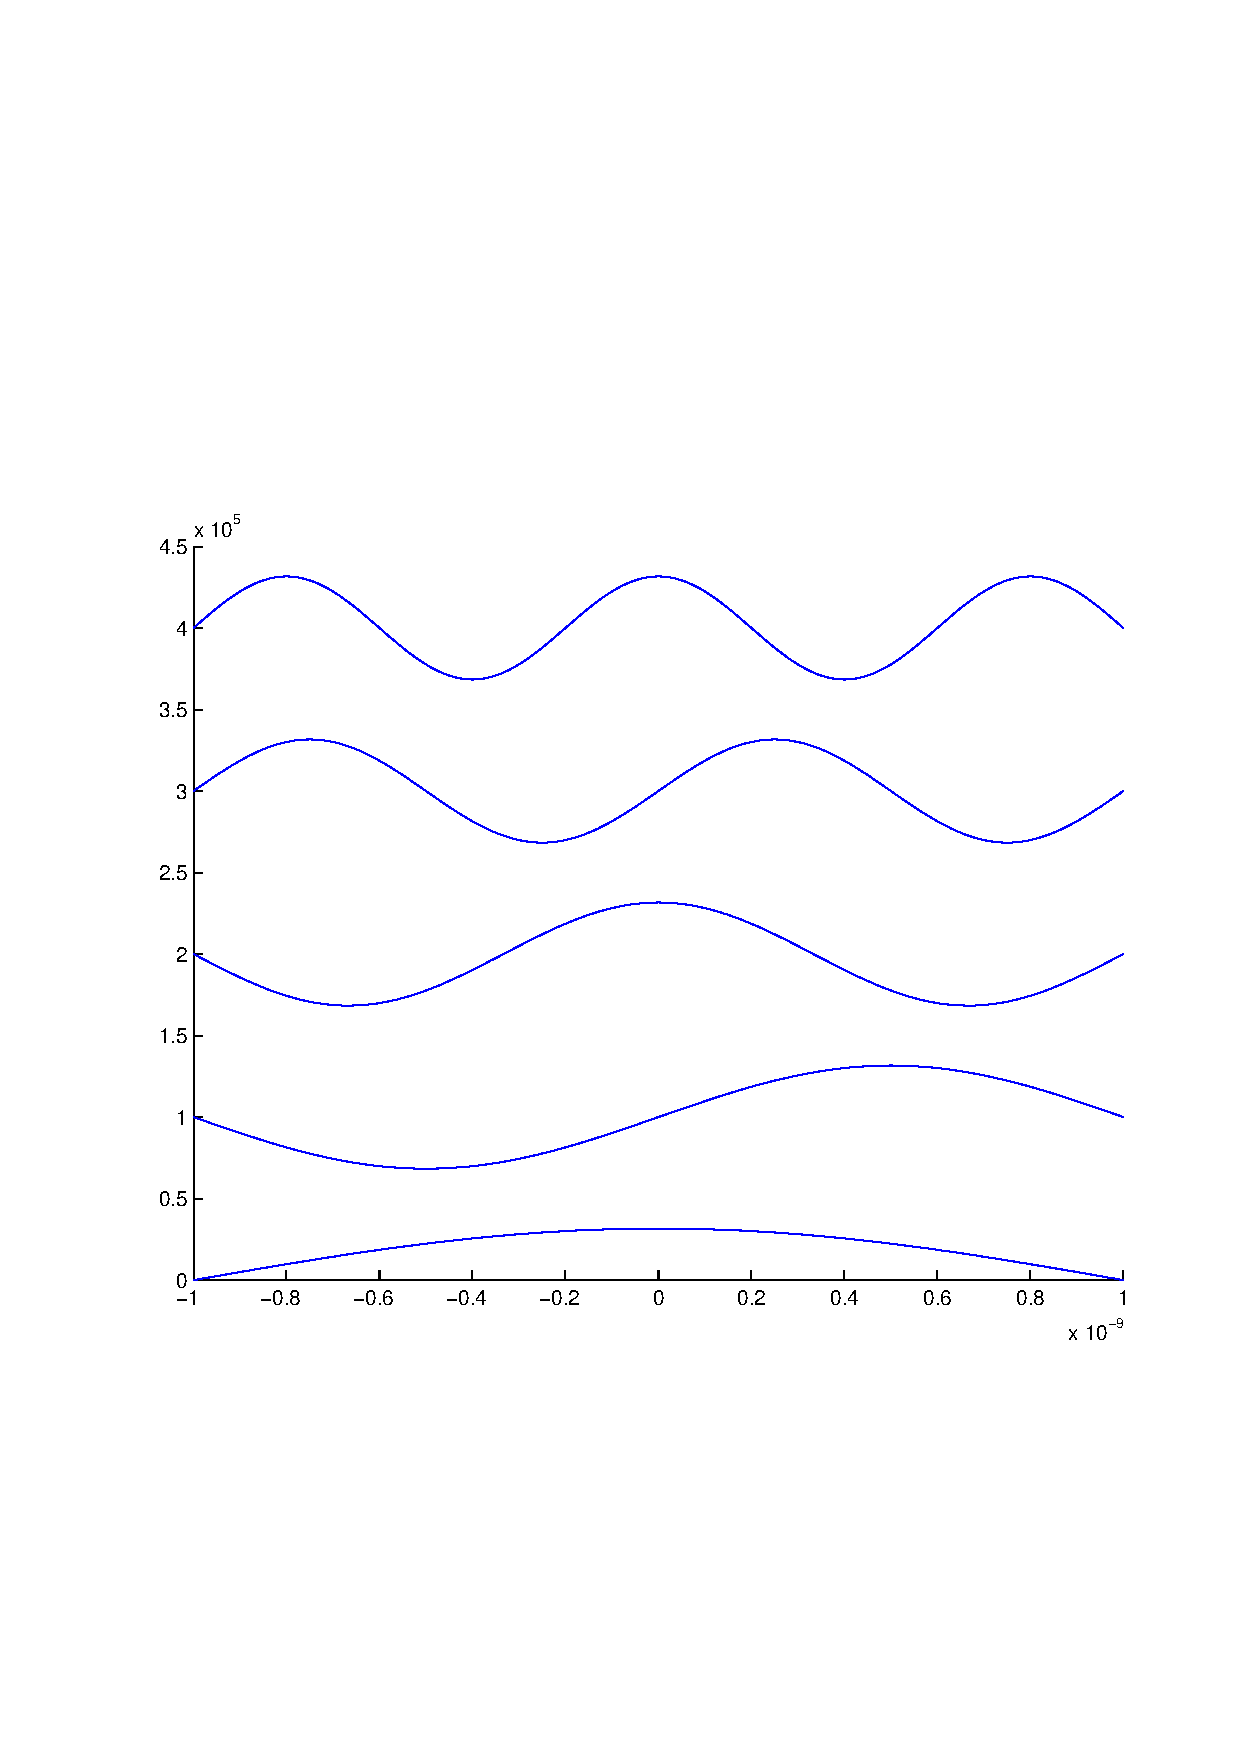
\includegraphics[width=12cm,clip=true,trim=2cm 7cm 1cm 8cm]{efeld/Psi_ungestoert.pdf}
 \caption{$\psi$ ungest\"ort}
 \label{abb:efeld_psi_ungestoert}
\end{figure}








\subsubsection{Berechnung 1. N"aherung}


Wir berechnen in diesem Beispie die erste N"aherung von einem Potentialskasten mit elektrischem Feld.
Dazu erweitern wir das einfache System  $\hat H_0$
(Siehe Abbildung \ref{skript:potentialkasten})
um $\hat H_1$, welcher die St"orung darstellt.
\[
  \hat{H} = \hat H_0 + \varepsilon \hat H_1
\]
F"ur $\hat H_0$ nehmen wir die Funktion aus dem Skript
\[
  \hat H_0 = \frac{\hbar^2}{2m} \frac{\partial^2}{\partial x^2} + V_0(x)
\]
wobei f\"ur das Potential $V_0(x)$ gilt
\begin{equation}
  \label{eq:efeld_v0_kasten}
  V_0(x)=\begin{cases}
    0       & \qquad |x|<l\\
    \infty  & \qquad\text{sonst.}
  \end{cases}
\end{equation}

$\hat H_1$ gibt unser elektrisches Feld an
\[
  \hat H_1 = a*x + b
\]
wir k"onnen $b = 0$ setzen da die Potenzials-Barriere unendlich gross ist und $a = 1$ weil wir die 
St"orung mit $\varepsilon$ steuern.
Die Ausgangsgleichung f\"ur $\hat{H}$ lautet somit:
\[
  \hat{H} = \varepsilon^0 ( \frac{\hbar^2}{2m} \frac{\partial^2}{\partial x^2} + V_0(x) )
            + \varepsilon^1*x
\]

Ausserdem ist das urspr"unglich $Psi_k^(0)$ gegeben.

\begin{equation}
\begin{aligned}
k&\ne l
&&\Rightarrow&
\langle\psi_l^{(0)}|\psi_k^{(1)}\rangle
&=
\frac{\langle \psi_l^{(0)}|\, H_1 \,|\psi_k^{(0)}\rangle}{E_k^{(0)}-E_l^{(0)}}
\\
k&=l
&&\Rightarrow&
E_k^{(1)}
&=
\langle \psi_k^{(0)}|\, H_1 \,|\psi_k^{(0)}\rangle
\end{aligned}
\end{equation}
\begin{equation}
|\psi_k(\varepsilon)\rangle
=
(1+i\varepsilon \gamma)
\,|\psi_k^{(0)}\rangle
+
\varepsilon
\sum_{k\ne l}
\frac{\langle \psi_l^{(0)}|\, H_1 \,|\psi_k^{(0)}\rangle}{E_k^{(0)}-E_l^{(0)}}
\,
|\psi_l^{(0)}\rangle
\end{equation}



In der Grafik \ref{abb:efeld_psi_gestoert} sehen wir die Unterschide zwischen dem normalen $\psi$ (schwarz) \& der ersten N"aherung (rot).

In diesem Beispiel haben wir die Unterschiede mit sehr starken Parmetern gew"ahlt.

Die einzelnen Werte in y-Richtung sind die jeweiligen N"aherungen. Alle Kurven pendeln um die 0-Achse.

\begin{figure}
 \centering
 \includegraphics[width=12cm,clip=true,trim=2cm 7cm 1cm 8cm]{efeld/Psi_gestoert.pdf}
 \caption{$\psi$ gest\"ort}
 \label{abb:efeld_psi_gestoert}
\end{figure}




\subsubsection{Energie "Anderung}

Was passiert?

In der Grafik \ref{abb:efeld_E_gestoert} lassen wir f"ur die jeweiligen stabilen Zust"ande 0..4 
den Einfluss der St"orung wachsen.

Da das elektrische Feld jedoch nur einen sehr kleinen Einfluss auf die gesammte Energie des 
Elektrons hat, mussten wir um die Effekte der 1. N"aherung zu zeigen ein sehr grosses $\varepsilon$
w"ahlen.

\begin{figure}
 \centering
 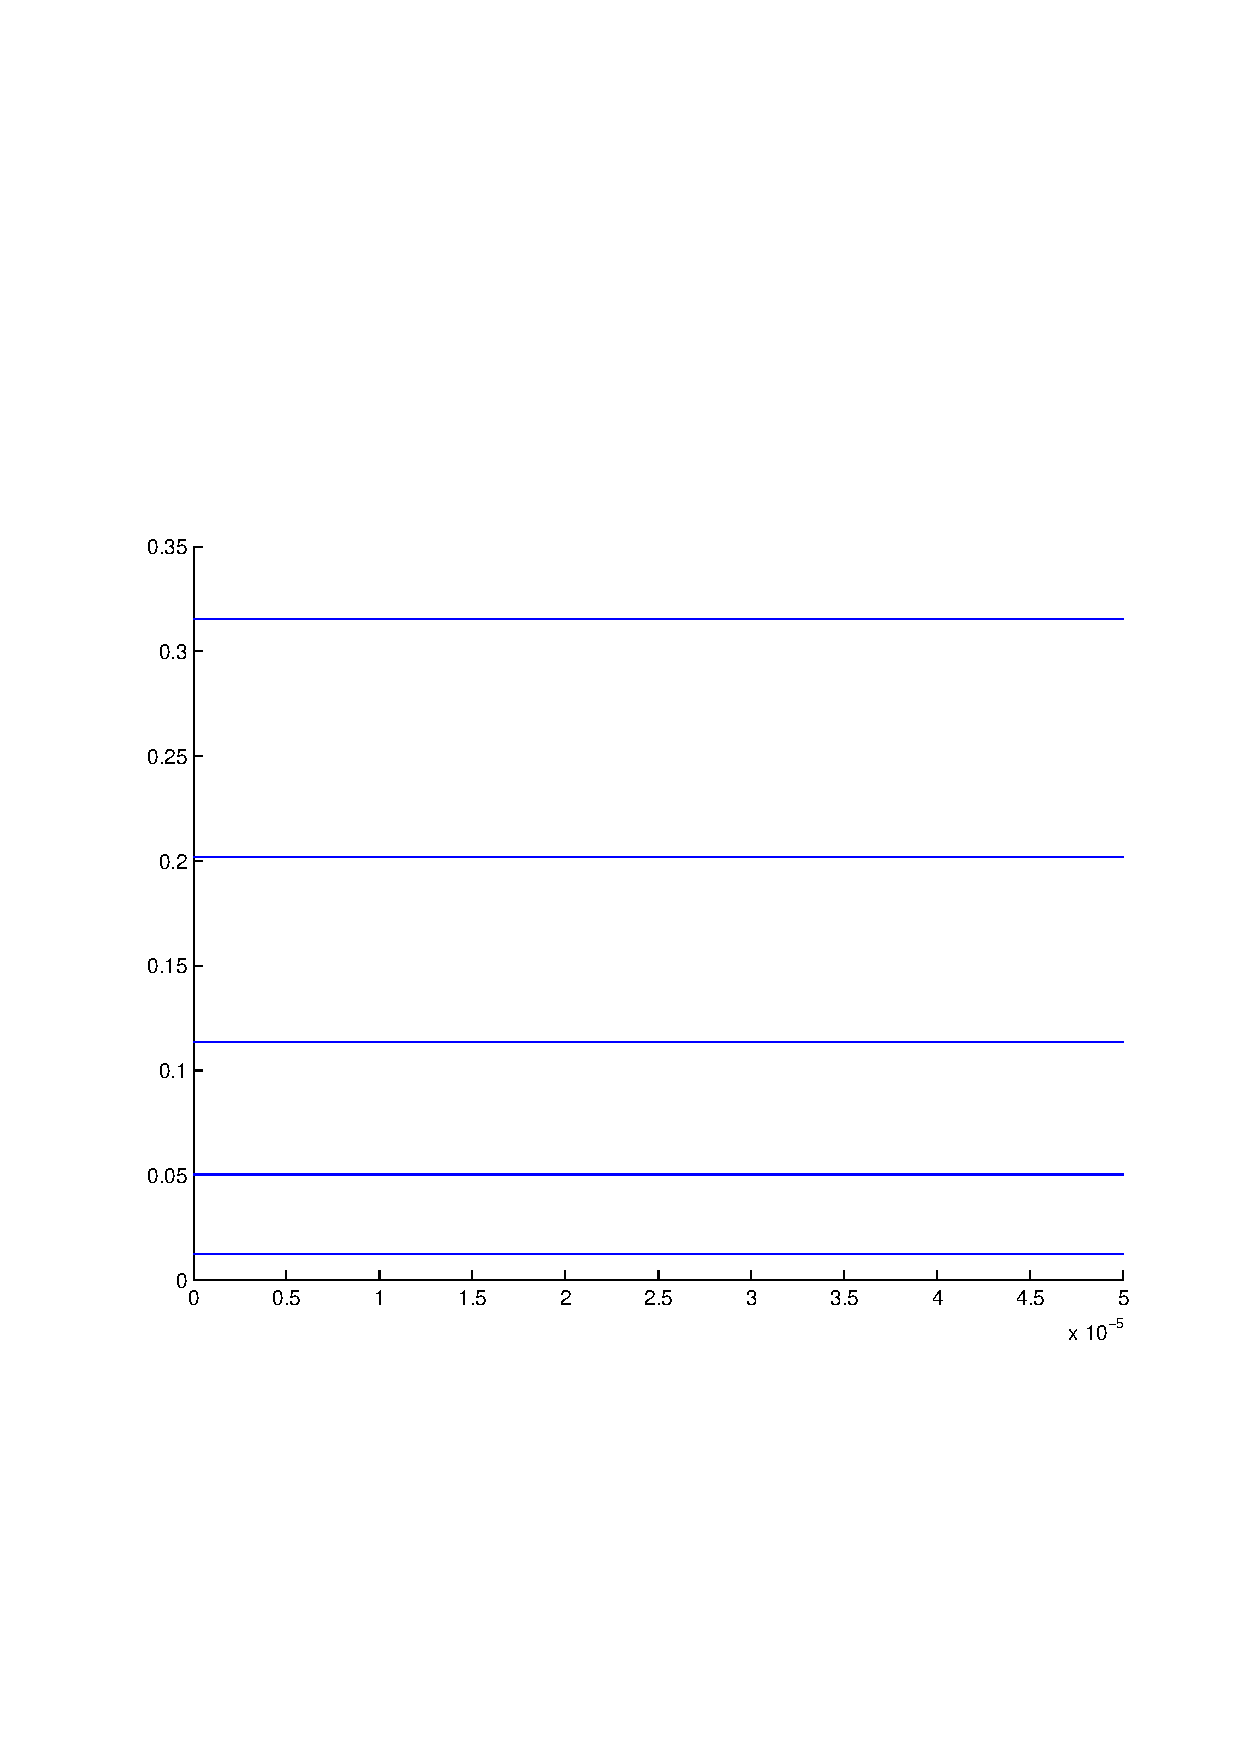
\includegraphics[width=12cm,clip=true,trim=2cm 7cm 1cm 8cm]{efeld/Energie_gestoert.pdf}
 \caption{$E$ gest\"ort, x-Achse ist $\varepsilon$, y-Achse ist die gesammte Energie des Systems}
 \label{abb:efeld_E_gestoert}
\end{figure}











\subsection{Potentialtopf}

In dieser Anwendung definieren wir das Potential ausserhalb von $l$ nicht mehr mit $\infty$, das Elektron kann mit gen"ugend Energie aus dem Topf gehoben werden.

\subsubsection{Berechnung 1. N"aherung}

Wir definieren den Potentialtopf basierend auf der Formel \ref{eq:efeld_v0_kasten}:
\begin{equation}
  V_0(x)=\begin{cases}
    0       & \qquad |x|<l\\
    1  & \qquad\text{sonst.}
  \end{cases}
\end{equation}

Wir "ubernehmen die St"orung aus der ersten Anwendung.
\[
  V_1 = x
\]


\printbibliography[heading=subbibliography]
\end{refsection}
